\documentclass{report}

\usepackage{tikz}

\pagestyle{empty}

\begin{document}
\begin{center}
    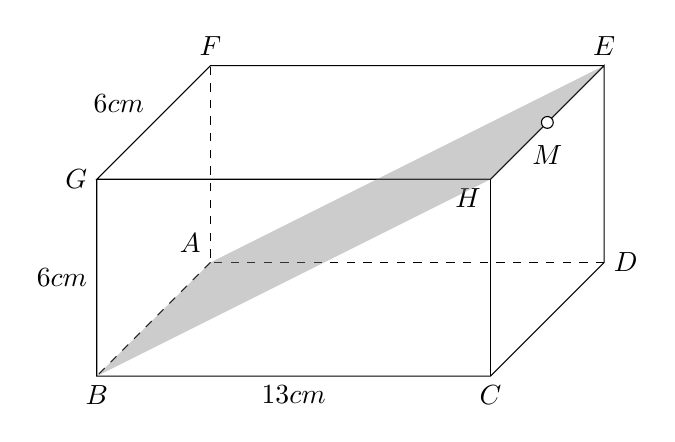
\begin{tikzpicture}[scale=2.5]
        \draw (2,1,0.5) node [above] {$E$} --(0,1,0.5) node [above] {$F$} --(0,1,2) node [left] {$G$} node [midway, above left] {$6cm$} --(2,1,2)node [below left] {$H$} --(2,1,0.5) --(2,0,0.5) node [right] {$D$} --(2,0,2) node [below] {$C$} --(0,0,2) node [below] {$B$} node [midway, below] {$13cm$} --(0,1,2) node [midway, left] {$6cm$};
        \draw (2,1,2)--(2,0,2);
        \draw[dashed](2,0,0.5)--(0,0,0.5) node [above left] {$A$}--(0,1,0.5);
        \draw[dashed](0,0,0.5)--(0,0,2);
        \fill [color=gray, opacity=0.4] (2, 1, 0.5) -- (2, 1, 2) -- (0, 0, 2) -- (0, 0, 0.5) -- cycle;
        \filldraw [black, fill=white] (2, 1, 1.25) circle [radius=0.03] node [below=5pt] {$M$};
    \end{tikzpicture}
\end{center}
\vspace{0.5cm}
\center{Page 181 Example 1}

\vfill\null{}
\begin{center}
    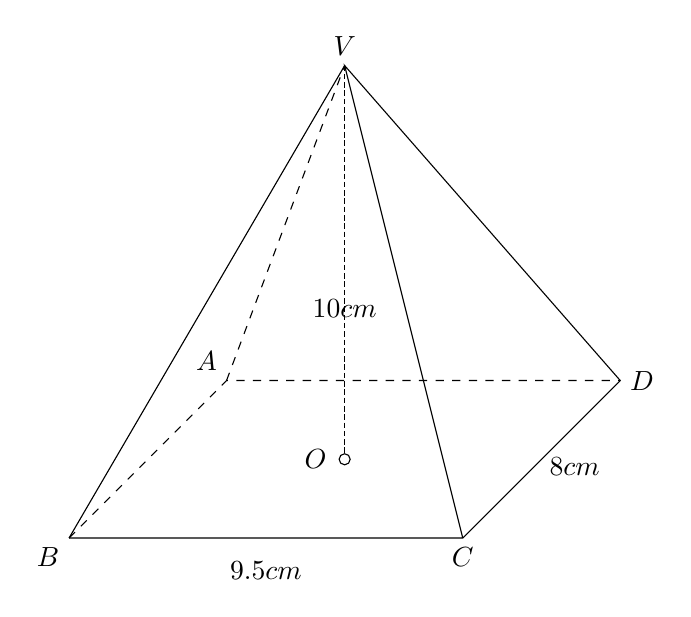
\begin{tikzpicture}[scale=2]
        \tikzstyle{point}=[circle,thick,draw=black,fill=black,inner sep=0pt,minimum width=4pt,minimum height=4pt]
        \node (a) at (0,0) {};
        \node (b) at (2.5,0) {};
        \node (c) at (3.5,1) {};
        \node (d) at (1,1) {};
        \node (e) at (1.75,3) {};
        \draw (a.center) node [below left] {$B$} -- (b.center) node [below] {$C$} node [midway, below=5pt] {$9.5cm$} -- (c.center) node [ right] {$D$} node [midway, right=12pt, below=-4pt] {$8cm$} -- (e.center) node [above] {$V$} -- (b.center);
        \draw (a.center) -- (e.center);
        \draw[dashed] (a.center) -- (d.center) -- (c.center);
        \draw[dashed] (d.center) node [above left] {$A$} -- (e.center);
        \node (f) at (1.75, 0.5) {};
        \draw[dash pattern=on 2pt off 1pt] (e.center) -- (f.center) node [left=3pt] {$O$} node [midway, below=10pt] {$10cm$};
        \filldraw[black, fill=white] (f.center) circle (1pt);
    \end{tikzpicture}
\end{center}
\vspace{0.5cm}
\center{Page 183 Example 3}

\newpage
\begin{center}
    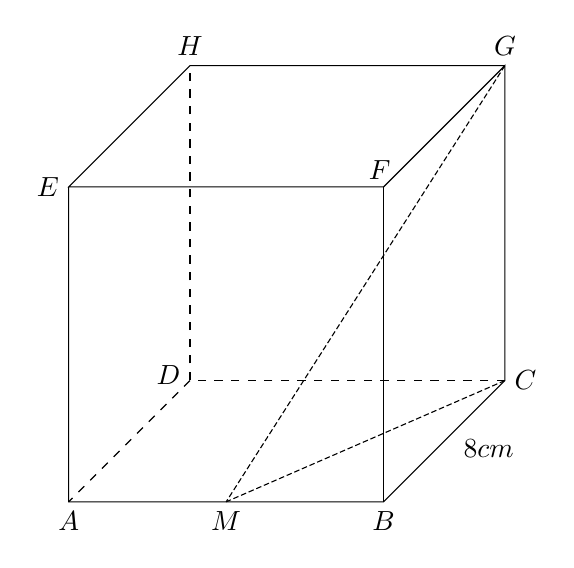
\begin{tikzpicture}[scale=2]
        \draw (2,2,0) node [above] {$G$} --(0,2,0) node [above] {$H$} --(0,2,2) node [left] {$E$} --(2,2,2) node [above=6pt, left=-6pt] {$F$} --(2,2,0)--(2,0,0) node [right] {$C$}--(2,0,2)node [below] {$B$} node [midway, right=16pt, below=-4pt] {$8cm$}--(0,0,2) node [below] {$A$}--(0,2,2);
        \draw (2,2,2)--(2,0,2);
        \draw[dashed](2,0,0)--(0,0,0)node [above=2pt, left] {$D$}--(0,2,0);
        \draw[dashed](0,0,0)--(0,0,2);
        \draw[dash pattern=on 2pt off 1pt] (2, 0, 0) -- (1,0,2);
        \draw[dash pattern=on 2pt off 1pt] (2, 2, 0) -- (1,0,2) node [below] {$M$};
    \end{tikzpicture}
\end{center}
\vspace{0.5cm}
\center{Page 172 Example 1}
\vfill\null{}
\begin{center}
    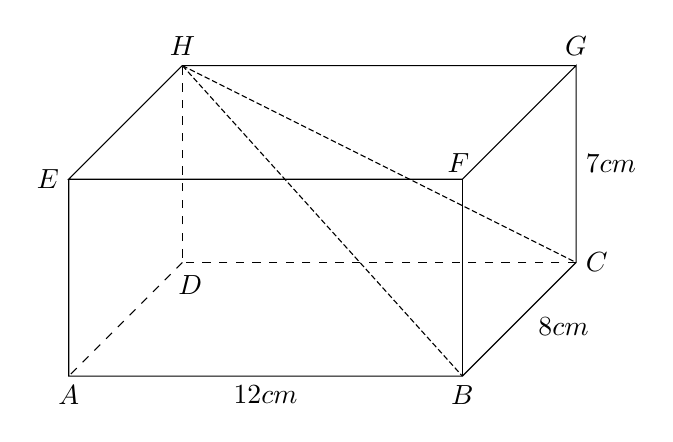
\begin{tikzpicture}[scale=2.5]
        \draw (2,1,0.5) node [above] {$G$} --(0,1,0.5) node [above] {$H$} --(0,1,2) node [left] {$E$} --(2,1,2) node [above=6pt, left=-6pt] {$F$} --(2,1,0.5)--(2,0,0.5) node [right] {$C$}  node [midway, right] {$7cm$}--(2,0,2)node [below] {$B$} node [midway, right=16pt, below=-4pt] {$8cm$} --(0,0,2)  node [midway, below] {$12cm$} node [below] {$A$}--(0,1,2);
        \draw (2,1,2)--(2,0,2);
        \draw[dashed](2,0,0.5)--(0,0,0.5)node [above=2pt, below=10pt, right=-5pt] {$D$}--(0,1,0.5);
        \draw[dashed](0,0,0.5)--(0,0,2);
        \draw[dash pattern=on 2pt off 1pt] (0, 1, 0.5) -- (2,0,0.5);
        \draw[dash pattern=on 2pt off 1pt] (0, 1, 0.5) -- (2,0,2);
    \end{tikzpicture}
    \vspace{0.5cm}
    \center{Page 174 Example 3}
\end{center}
\end{document}